We will be talking about the implementation/tags used in XML-FOto have a general idea of what XSL-FO is necessary.

\subsection{Introduction}


XSL formatting objects. XSL-FO stands for Extensible Stylesheet Language Formatting Objects. This is a format used to format pages for example html or some other format. XML-FO is primarily a generated format. In most cases you have an XML,XSLT and CSS and you will generate the XML-FO.
\subsection{Formatting}

XSL-FO documents contain two required sections. The first section details a list of named page layouts. The second section is a list of document data, with markup, that uses the various page layouts to determine how the content fills the various pages. All output (text, pictures, etc.) will be formatted into boxes and then displayed or printed to a target media.1). The main class in a XSL is a page master. This is a required section that defines the layout. Pages can be divided in regions. The main regions are

\begin{enumerate}
	\item region-body (the body of the page)
    \item region-before (the header of the page)
    \item region-after (the footer of the page)
    \item region-start (the left sidebar)
    \item region-end (the right sidebar)
\end{enumerate}


Each of these regions contain \textbf{block areas}. The block areas can be contain other block areas or plain text or other kinds of formatting like a list or table. Each page master needs to have an unique name. With this you can define different standard layouts for different kinds pages. Some of the things that can be defined in a page master are: the size of the pages and the margins of the given regions. More importantly, it can define sequences of pages that allow for effects where the odd and even pages look different The flow tag specifies what will be outputted to the page. The tag for the is fo:sequence this defines an output page. Each output page refers to a master page which defines the layout. The flow tags will output in the data in sequence. The flow tag can be used within each of the regions which have been specified before. Within the flow tag you will define a block where you will put in your data.2). So output is mostly nested inside <fo:block> elements, nested inside <fo:flow> elements, nested inside <fo:page-sequence> elements

\subsection{Features of XSL-FO} 
\begin{enumerate}
	\item Multiple columns
    \item Lists
    \item Footnotes
    \item Miscellaneous
    \item Page number citations. A page that contains a special tag can be cited in text, and the FO processor will fill in the actual page number where this tag appears.
    \item Ordered List ItemBlock borders, in a number of styles.
    \item Background colors and images.
    \item Font controls and weighting, as in CSS.
    \item Side floats.
    \item Miscellaneous Inline Elements.
    \item Multiple flows and flow mapping
\end{enumerate}
    

XSL-FO 1.0 was fairly restrictive about what text was allowed to go in what areas of a page. Version 1.1 loosens these restrictions significantly, allowing flowing text to be mapped into multiple explicit regions on a page. This allows for more newspaper-like typesetting.

\begin{enumerate}
    \item Bookmarks
    \item Indexing
    \item Last page citation
    \item Table markers
    \item Inside/outside floats
\end{enumerate}

\subsection{Required components of an FO file} 
\begin{itemize}
\item XML Declaration
\begin{lstlisting}[language=xml]
<?xml version="1.0" encoding="utf-8"?>
\end{lstlisting}


\item Root Node (contains whole document including page layout and document data, declares namespace)
\begin{lstlisting}[language=xml]
<fo:root xmlns:fo="http://namespace.com">
    <!--Page layout goes here-->
    <!--Document data goes here-->
</fo:root>
\end{lstlisting}

\item Page Layout (defines the properties of a page including the size, margins, direction of the text flow) 
\begin{figure}
\label{fig:layoutxmlfo}
\caption{Page layout for XML fo}
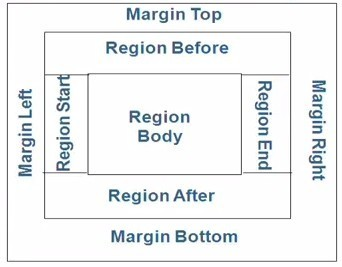
\includegraphics[origin=c]{images/layoutxmlfo.jpg}
\end{figure}
\begin{lstlisting}[language=xml]
<fo:layout-master-set>
<fo:simple-page-master master-name="A4" page-width="297mm"
page-height="210mm" margin-top="1cm" margin-bottom="1cm"
margin-left="1cm" margin-right="1cm">
  <fo:region-body margin="3cm"/>
  <fo:region-before extent="2cm"/>
  <fo:region-after extent="2cm"/>
  <fo:region-start extent="2cm"/>
  <fo:region-end extent="2cm"/>
</fo:simple-page-master>
</fo:layout-master-set>
\end{lstlisting}
\item Document Data
\begin{lstlisting}[language=xml]
<fo:page-sequence>
  <fo:flow flow-name="xsl-region-body">
    <fo:block>
      <!-- Output goes here -->
    </fo:block>
  </fo:flow>
</fo:page-sequence>
\end{lstlisting}
\begin{figure}[h]
\label{fig:fo2}
\caption{Page layout for XML fo}
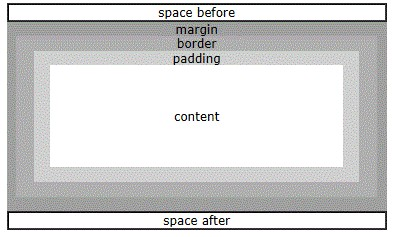
\includegraphics[origin=c]{images/fo2.jpg}
\end{figure}
\end{itemize}
\subsection{Tables in XML FO}
\begin{lstlisting}[language=xml]
<fo:page-sequence master-reference="mainPage">
     <fo:flow flow-name="xsl-region-body">
        <fo:block font-size="28pt" line-height="36pt" padding-after="12pt">
                Creating XSL-FO Tables
        </fo:block>
     <fo:table width="16cm" table-layout="fixed">
     <fo:table-column column-number="1" column-width="30mm">
     </fo:table-column>
     <fo:table-column column-number="2" column-width="30mm">
     </fo:table-column>
     <fo:table-column column-number="3" column-width="30mm">
     </fo:table-column>
     <fo:table-body>
  <fo:table-row line-height="26pt">
         <fo:table-cell column-number="1" border-style="solid">
              <fo:block font-family="sans-serif" font-size="20pt" font-weight="bold"> State</fo:block>
       </fo:table-cell>
    </fo:table-row>
 </fo:table-body>
 </fo:table>
 </fo:flow>
</fo:page-sequence>
\end{lstlisting}
\begin{tabular}{|l|l|l|}
\hline
This & is & a \\ \hline
table & in & latex \\ \hline

\end{tabular}
\cite{informit} 
\subsection{Lists in XML FO}
\begin{lstlisting}[language=xml]
<fo:page-sequence master-reference="mainPage">
<fo:flow flow-name="xsl-region-body">
<fo:block font-size="28pt" line-height="36pt">
Creating XSL-FO Lists
</fo:block>
fo:list-block
provisional-distance-between-starts="10mm"
provisional-label-separation="5mm" font-size="36pt">
   <fo:list-item line-height="24pt">
   <fo:list-item-label>
   <fo:block font-family="sans-serif" font-size="18pt"> 1. </fo:block>
   </fo:list-item-label>
         <fo:list-item-body start-indent="body-start()">
            <fo:block font-family="sans-serif"font-size="18pt">No</fo:block>
    </fo:list-item-body>
    </fo:list-item>
  </fo:list-block>
 </fo:flow>
</fo:page-sequence>
\end{lstlisting}

Document data always starts with $<fo:page-sequence>$ tag. After that “flow” tag defines which part of the page will be used. Blocks can contain tables, lists, inline elements

Basically; XSL-FO output is normally nested inside $<fo:block>$ elements, nested inside $<:flow>$ elements, nested inside $<fo:page-sequence>$ elements 